
An alternate method for fusion of redundant sensors is proposed that is similar to voting algorithms employed by Flight Control Systems of \cite{tischler_advances_2018}. An issue for voting algorithms is the abrupt exclusion of single sensors once their difference to the other sensors is too large. Hence, a weighting strategy for averaging is proposed that is based on the value difference.

An example is shown in figure \ref{fig:fusing_method}

This method tries to account dynamically for sensor distance by scaling parameters to small values compared to their neighbours. This works for a minimum of three redundant values.

Based on the single sensor values a distance matrix for $d_{i,j}$ is set up.

% Please add the following required packages to your document preamble:
% \usepackage{booktabs}
\begin{table}[]
    \begin{tabular}{@{}llll@{}}
        \toprule                 & A    & B    & C    \\ \midrule
        \multicolumn{1}{l|}{A}   & 0    & 0.25 & 2    \\
        \multicolumn{1}{l|}{B}   & 0.25 & 0    & 1.75 \\
        \multicolumn{1}{l|}{C}   & 2    & 1.75 & 0    \\ \midrule
        \multicolumn{1}{l|}{Sum} & 2.25 & 2    & 3.75 \\ \bottomrule
    \end{tabular}
\end{table}

The column sum is then further defined $\hat{d_{i}}$. To generate a ratio we define:

\begin{equation}
    w_i=\frac{1}{\hat{d_i}}
    \label{eq:fusing_weight}
\end{equation}

Since we desire that
$\sum{w_i}\overset{!}{=}1$ we need to scale the ratios using:

\begin{equation}
    \bar{w_{i}} = \frac{w_i}{\sum{w_i}}
\end{equation}


With this ratio we can now calculate the new fused value:

\begin{equation}
    \bar{x} = \sum_{i}^{n} x_i \cdot \bar{w_{i}}
\end{equation}

This works out to a fused value that is shown in \ref{fig:fusing_algo}.

Compare results with averaging here using figure.

To further increase sensitivity for distance we can replace the term in equation \ref{eq:fusing_weight} with a quadratic term:
\begin{equation}
    w_i=\frac{1}{\hat{d_i}^2}
\end{equation}

















\subsubsection{Examining Altitude Sensors}
%byeeee. sorry context was not relevant anymore
As seen in~\ref{fig:gps_diff} gps altitudes have a base mean value of difference of about 3-4 meters. During flight level changes the base level changes significantly. Further investigation is needed how these changes may arise.

One possible approach would be considering different placements of gps antennas within the airframe. since the IMAR's position is precisely known and lies around the center of gravity but the ASCB's gps position is not known exactly the process is not facilitated. However using the process of lever arms the position could be roughly estimated and compensated from the altitude difference in figure \ref{fig:gps_diff}.

\begin{figure}[h]
    \centering
    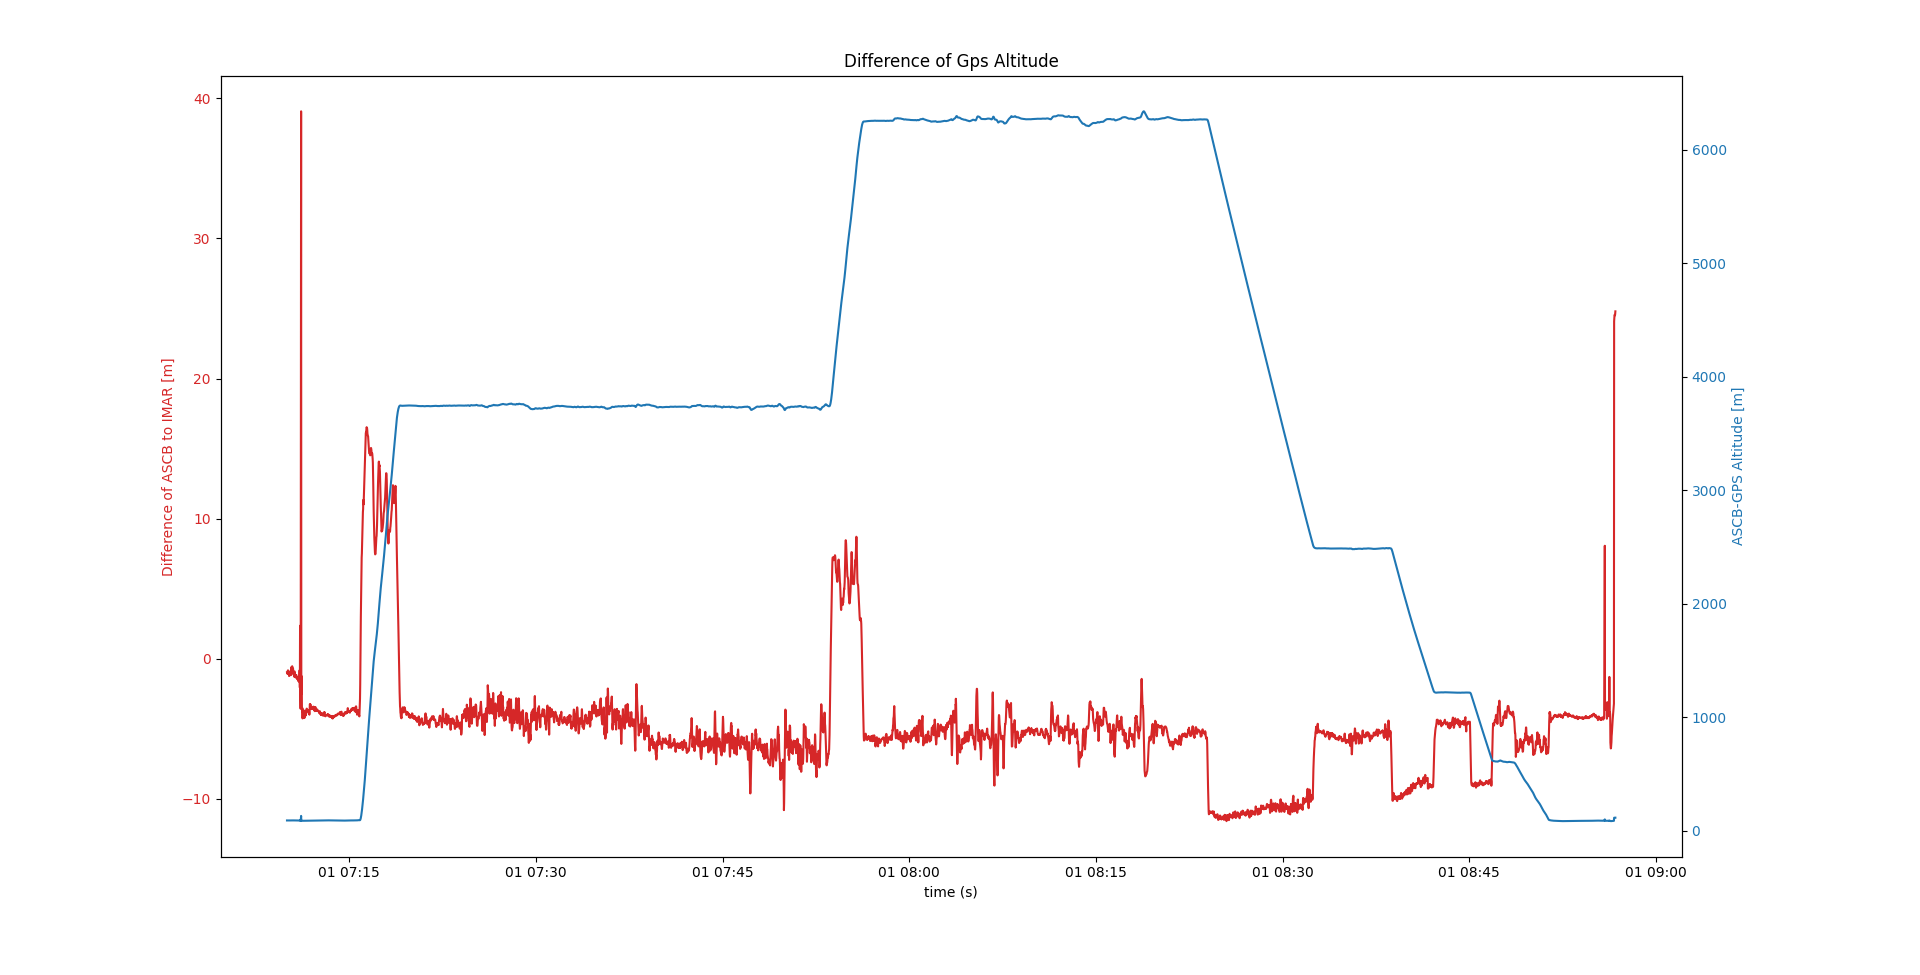
\includegraphics[width=.8\textwidth]{gps_difference_imar_ascb}
    \caption{Comparing the GPS sensors from the internal aircraft GPS (ASCB) to an experimentally installed GPS system (IMAR)}
    \label{fig:gps_diff}
\end{figure}

Another incurring deviation is investigating the ~40m/150ft offset for gps altitudes. Possible causes may be Uncorrected Ellipsoid gnss altitudes. However, this appears unlikely since generally the offset in the region would be added and not subtracted [further investigation needed].


Difficulty diagnosing sensors without previous knowledge. limitations within sensor behaviour. Checks include: range, too much sensor movement, too few sensor movement.

Relative examinations possible for errors occuring for finite time within experiment but not if all of the experiment data is corrupt.

\paragraph{Altitude Comparison}

plot here: -gps to gps -gps to baro. Beta overlayed as well as Ma Number




some mean ground has to be found to crossreference the various altitudes.

For standardization. The SI-unit meters is used for altitudes.

In the first draft. The altitude is sampled with 1Hz for computational speed and since gnss update rates are updated in a similar frequency.

\paragraph{ Physical}

\paragraph{ GNSS}

The following briefly glosses over GNSS and does not delve into the technical details. it rather tries to present GNSS Systems as a black box and examines inputs and outputs.

Generally speaking, GNSS systems calculate position based on run times to satellites. For output GNSS systems return position values for the ellipsoid model of the earth. Since the difference between MSL and ellipsoid varies for up to 100m vertically based on the receivers positions on the earth. Mostly, the difference is in the 40-50m range in germany.

Explain here why orthometric and ellipsoid value differs (vector difference, cg)

GNSS-units work with geoid models to deliver an orthometric value. Different Geoid models have different drawbacks and resolutions. For aviation use, the World Geodetic System (WGS84) generally proposes a geoid model that is used. Within this works scope it is omitted to implement an existing geoid model into the software-loop to reserve this workload for a later time.
